\section{Question 1: Workload structure and capacity pressure}
\label{sec:r1q1}
The supplied trace has 224,112 jobs on 4,278 nodes, with 10,412 GPUs and 632,636 vCPUs across six GPU models. For job $j$, $a_j$ is release time, $p_j$ duration, $W_j$ workers, and $(g_j,c_j)$ the per-worker GPU and vCPU requests. Submitted GPU work is $H_j=W_jg_jp_j$; it is a request-based quantity, not measured device utilization. The six model pools have distinct capacities and request shapes; their formal simulated outcomes are reported with the scheduler evidence in Question~2. The exact input hashes and the serialization comparison are in the provenance record, so the claims below use the formal-run CSV.

\begin{table}[H]
\centering
\caption{Workload type statistics from the formal raw CSV. Percentages are jobs or submitted GPU-work as labelled; the multi-worker summary reports counts and the median/P95/maximum worker count.}
\label{tab:r2q1types}
\setlength{\tabcolsep}{2.5pt}
\begin{tabularx}{\linewidth}{l>{\raggedright\arraybackslash}X>{\raggedright\arraybackslash}X>{\raggedright\arraybackslash}X}
\toprule
Population & Duration $\le 1$ h (jobs; GPU-work) & Duration $>24$ h (jobs; GPU-work) & Worker structure \\
\midrule
All 224,112 & 70.751\%; 0.721\% & 9.295\%; 92.350\% & $W=1$: 90.953\%; $W>1$: 20,276 jobs (9.047\%). Within multi-worker: $W=2$--8: 16,559; $W\ge9$: 3,717; median/P95/max $=4/28/249$. \\
A10 111,284 & 79.035\%; 0.176\% & 10.717\%; 99.417\% & $W=1$: 99.293\%; $W>1$: 787 jobs (0.707\%). Within multi-worker: $W=2$--8: 637; $W\ge9$: 150; median/P95/max $=4/17.7/60$. \\
\bottomrule
\end{tabularx}
\end{table}

\begin{figure}[H]\centering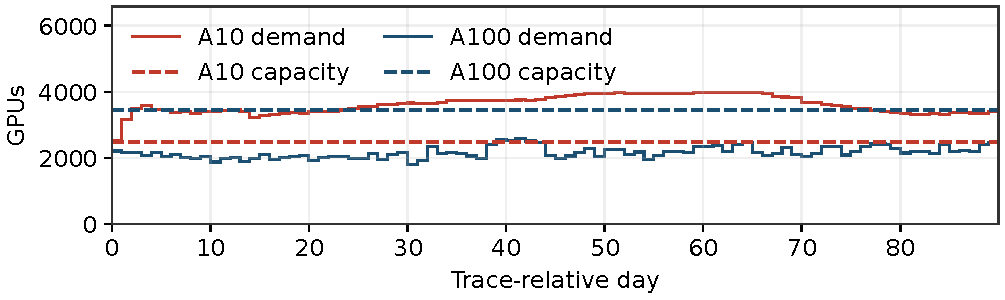
\includegraphics[width=\linewidth]{r1_figures/fig1_demand.pdf}\caption{Exact daily-bin overlap of the immediate-start counterfactual and physical GPU capacity. This is demand/capacity, not simulated allocation. The A10 mean is 3,614.54 GPUs against 2,494 capacity and its peak is 4,103; A100 demand stays below its 3,456-GPU capacity.}\label{fig:r1demand}\end{figure}

The workload is concentrated: GPU-work Gini is 0.9522, the top 1\% (2,241 jobs) contributes 43.30\%, and the top 5\% (11,205 jobs) contributes 87.68\%. Median duration is 1,330 s, the 95th percentile is 309.09 h, and the maximum is about 184 days. There are 3,512 jobs at trace time zero; without a calendar origin, their position is reported as a trace-origin batch rather than a weekday effect. The exposure-corrected relative 24-hour profile peaks at phase hour 16 and is lowest at hour 4 (ratio 2.29); this is a relative phase diagnostic, not a timezone claim.

The shape is also strongly single-worker: 90.95\% of jobs use one worker, 78.42\% use one GPU per worker, and the means are 1.539 workers and 2.003 GPUs per worker. Daily arrivals are nonstationary at the trace scale: the first day contains 8,509 jobs, day 1 contains 5,525, and the minimum is 965 jobs on day 63. These counts describe the observed window and do not identify a calendar effect or a particular arrival process.

\begin{figure}[H]\centering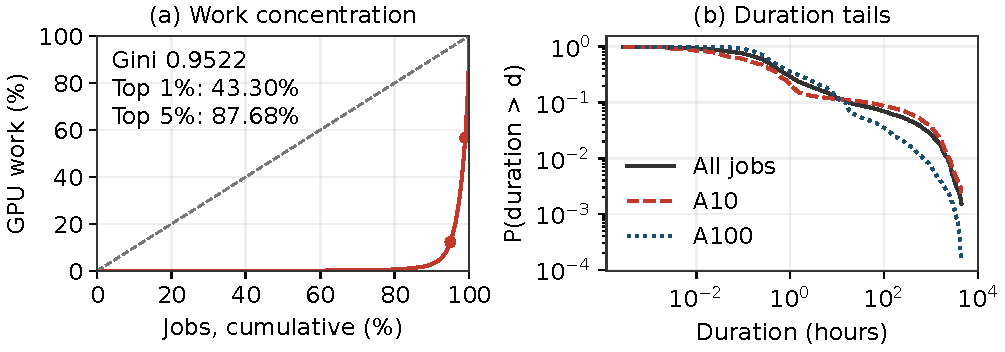
\includegraphics[width=\linewidth]{r1_figures/fig1_data_patterns.pdf}\caption{Two high-information views of the formal data: cumulative GPU-work concentration and strict duration tails.}\label{fig:r1patterns}\end{figure}

For model $m$, with exact Q1 observation window $T=7,775,878$ s, the lifetime-work ratios are
\begin{equation}
\rho_m^{GPU}=\frac{\sum_{j\in\mathcal J_m}W_jg_jp_j}{T\sum_{i\in\mathcal I_m}G_i},\qquad
\rho_m^{CPU}=\frac{\sum_{j\in\mathcal J_m}W_jc_jp_j}{T\sum_{i\in\mathcal I_m}C_i}.
\end{equation}
A10 has $\rho^{GPU}=2.064$, while GPU-series-1 has a shape mismatch: 2,478 jobs (25.70\% of that pool, 78.07\% of its work) exceed the 24-vCPU/GPU ratio of its 8-GPU, 192-vCPU nodes. The 24-, 48-, 128- and 192-vCPU/GPU configurations contain 77, 10, 1 and 901 nodes respectively. This motivates node-level gang checks; it does not identify a unique bottleneck policy.
